\documentclass{scrbook}
\usepackage{graphicx} % Required for inserting images
\usepackage{tabularx} % Required for fixed width tables
\usepackage{scrlayer-scrpage} % Required for the subtitles
\usepackage{url} % Required for the URLs
\usepackage{hyperref} % Required for the URLs
\usepackage{listings} % Required for the code snippets
\usepackage{mathtools} % Required for the system of equations

\usepackage{fontspec}
\setmonofont{DejaVu Sans Mono} % Overleaf has this font pre-installed

% Put the caption of the snippets at the bottom
\lstset{
    captionpos=b,
    basicstyle=\ttfamily\small,
    columns=fullflexible,
    keepspaces=true
}


\title{JavaScript}
\subtitle{Ambient intelligence course (A.Y. 2025/2026)\\Topic taught by Prof. Davide Loconte}
\author{Gabriele Colapinto}
\date{\today}

\begin{document}

\maketitle
\thispagestyle{empty}

{\Large\textbf{License}} \\
{Notes from Ambient intelligence (A.Y. 2025/2026) by Gabriele Colapinto. 
Course taught by professors Michele Ruta, Floriano Scioscia, Arnaldo Tomasino, Davide Loconte — 
Licensed under CC BY-NC 4.0.\\
\url{https://creativecommons.org/licenses/by-nc/4.0/}}

\vspace*{\fill}
\rule{\textwidth}{0.2pt}
\small{© 2025 Gabriele Colapinto \\
Released under the \href{https://creativecommons.org/licenses/by-nc/4.0/}{Creative Commons Attribution–NonCommercial 4.0 International License}}

\clearpage

\tableofcontents

\chapter{Core Concepts and Programming Paradigm}

JavaScript is a dynamically typed, platform-independent scripting language designed for client-side execution within a web browser. Introduced in 1995 with Netscape Navigator 2.0, its strategic importance lies in its ability to transform static web pages into active, interactive user experiences. As a core technology of the web, JavaScript works alongside HTML and CSS to provide the dynamic behavior that defines modern applications. Despite the name, JavaScript is not related to the Java programming language. Unlike many traditional languages, it is built on a prototype-based object-oriented paradigm, a foundational concept that shapes how data and behavior are structured. \\

A key distinction in object-oriented languages is the difference between class-based and prototype-based models. Mainstream languages like Java and C++ use a class-based system, whereas JavaScript employs a prototype-based approach. It's important to note that while modern JavaScript includes a \texttt{class} keyword for a more familiar syntax, this is merely "syntactic sugar" over the underlying prototype system and does not change its fundamental paradigm. The core differences are summarized below:

\begin{table}[h!]
    \begin{tabularx}{\linewidth}{|X|X|X|}
        \hline
        Paradigm & Entity Model & Property Inheritance \\ \hline
        
        \textbf{Class-based (e.g., Java, C++)} &
        Based on two distinct entities: \textbf{classes} (blueprints) and \textbf{instances} (objects created from the blueprint). A class defines the properties and methods for a set of objects. &
        An instance inherits properties directly from the class it was created from. The class acts as the single template. \\ \hline
        
        \textbf{Prototype-based (JavaScript)} &
        Based on a single entity: the \textbf{object}. There is no formal distinction between a class and an instance. &
        A new object inherits properties from another object that serves as its \textbf{prototype}. Any object can act as a template for another. \\ \hline
    \end{tabularx}
\end{table}

Modern web browsers execute JavaScript code using sophisticated engines, such as Google's V8 (used in Chrome) and Mozilla's SpiderMonkey (used in Firefox). These engines do not simply interpret code line-by-line. Instead, they employ a process known as \textbf{Just-In-Time (JIT) compilation}. This technique compiles JavaScript into executable machine code at runtime, making execution significantly more efficient and faster than traditional interpretation.

\section{JavaScript Engine: AST, Bytecode, JIT, and De-optimization}

\begin{figure}
    \centering
    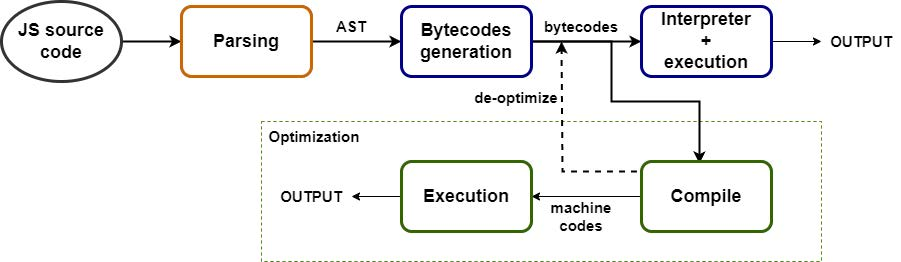
\includegraphics[width=\linewidth]{Images/How_JavaScript_engines_work.jpg}
    \caption{JavaScript engine compilation pipeline}
    \label{fig:javascript_engine_compilation_pipeline}
\end{figure}

Figure \ref{fig:javascript_engine_compilation_pipeline} illustrates the execution pipeline of a modern JavaScript engine (e.g., V8), which combines interpretation and Just-In-Time (JIT) compilation to achieve both fast startup and high performance.

\subsection{Abstract Syntax Tree (AST)}

After parsing, the JavaScript source code is transformed into an \textbf{Abstract Syntax Tree (AST)}. It is called ``abstract'' because it represents the logical structure of the program while omitting irrelevant syntactic details such as whitespace, formatting, or redundant parentheses.\\

For example:

\begin{lstlisting}
    1 + 2 * 3
\end{lstlisting}

is represented as a tree where nodes correspond to operations and operands, reflecting operator precedence.

\begin{lstlisting}
    +
   / \
  1   *
     / \
    2   3
\end{lstlisting}

The AST captures the semantics of the program rather than its textual form.

\subsection{Bytecode Generation}

From the AST, the engine produces \textbf{bytecode}, an intermediate representation that is closer to execution than source code but still independent of the underlying hardware.\\

The bytecode:
\begin{itemize}
    \item is \textbf{engine-specific} (e.g., V8 bytecode),
    \item is \textbf{independent of the operating system and CPU},
    \item enables portability across platforms running the same engine.
\end{itemize}

\subsection{Interpretation}

Initially, the bytecode is executed by an \textbf{interpreter}. This allows the program to start quickly without the overhead of compiling everything upfront. The interpreter executes instructions one by one, which is flexible but slower than native execution.

\subsection{Just-In-Time Compilation (JIT)}

To improve performance, modern engines monitor execution and identify \textbf{hot code}, i.e., portions of the program that are executed frequently (such as loops or frequently called functions).\\

These parts are compiled into \textbf{machine code} by a JIT compiler. The compiled code runs significantly faster than interpreted bytecode.\\

The selection of code to compile is based on heuristics such as:
\begin{itemize}
    \item execution frequency,
    \item stability of observed types,
    \item predictability of control flow.
\end{itemize}

\subsection{Speculative Optimization}

JIT compilation relies on \textbf{speculative assumptions}. For instance, if a function is repeatedly called with numeric arguments, the compiler may generate optimized machine code assuming numeric types only.\\

These optimizations include:
\begin{itemize}
    \item type specialization,
    \item function inlining (inlining = embedding directly within HTML),
    \item inline caching,
    \item optimized object access.
\end{itemize}

\subsection{De-optimization}

If a speculative assumption is violated (e.g., a function previously called with numbers is later called with strings), the optimized machine code may no longer be valid.\\

In this case, the engine performs \textbf{de-optimization}:
\begin{itemize}
    \item execution falls back to the interpreter,
    \item a more general (less optimized) version of the code is used.
\end{itemize}

This explains the feedback loop shown in the figure, where compiled code can return to interpreted execution.

\subsection{Coexistence of Interpreted and Compiled Code}

Interpreted and compiled code can coexist seamlessly. Different parts of the same program may be:
\begin{itemize}
    \item interpreted,
    \item compiled and optimized,
    \item de-optimized and reinterpreted.
\end{itemize}

This does not introduce inconsistencies because the engine preserves the same JavaScript semantics across all execution modes.

\subsection{Concurrency and External Interactions}

The presence of JIT compilation does not affect the concurrency model of JavaScript. The language remains:
\begin{itemize}
    \item single-threaded (based on the event loop),
    \item asynchronous for I/O operations.
\end{itemize}

Therefore, concerns such as race conditions or external interactions (e.g., network requests) are not impacted by whether code is interpreted or compiled.

\subsection{Platform Dependence}

While bytecode and optimization strategies are largely platform-independent, the final \textbf{machine code} generated by the JIT compiler is platform-specific.\\

Thus:
\begin{itemize}
    \item the overall execution strategy is consistent across platforms,
    \item low-level optimizations may vary depending on the CPU architecture.
\end{itemize}

With this conceptual background established, we can now move to the practical steps of embedding and writing JavaScript code within a standard web page.

\chapter{Syntax and Integration with HTML}

To bring a web page to life with JavaScript, the code must be embedded within an HTML document. The browser's JavaScript engine will then discover and execute this code as it parses the page. This section provides the practical foundation for writing and executing your first lines of JavaScript.\\

There are two primary methods for including JavaScript in an HTML file:

\begin{enumerate}
    \item
    \textbf{Internal Script:} You can write JavaScript code directly within an HTML document by placing it inside a \texttt{<script>} tag. This is suitable for small, page-specific scripts.
    \begin{lstlisting}
        <script type="text/javascript">
            ... JavaScript code ...
        </script>
    \end{lstlisting}
    
    \item
    \textbf{External Script:} For better organization and code reuse, JavaScript can be placed in a separate file with a \texttt{.js} extension. This file is then linked to the HTML document using the \texttt{src} attribute of the \texttt{<script>} tag. This approach is highly recommended as it separates structure (HTML) from behavior (JavaScript), improving maintainability.
    \begin{lstlisting}
        <script type="text/javascript" src="myfunctions.js"/>
    \end{lstlisting}
\end{enumerate}

To provide a fallback for users who have disabled JavaScript in their browsers, or for non-interactive user agents like \textbf{printers} that cannot execute code, the \texttt{<noscript>} tag is used. The content inside \texttt{<noscript>} is displayed only when scripts are not supported or are disabled.

\begin{lstlisting}[language=html]
<noscript>
  <p>
    This website requires JavaScript to be enabled for full functionality.
  </p>
</noscript>
\end{lstlisting}

JavaScript's syntax is heavily influenced by C-like languages and each segment of JS code is formed by one or more statements. Key syntactical rules include:

\begin{itemize}
    \item
    Statements can be separated by a semicolon (\texttt{;}), although a line break is often sufficient to mark the end of a statement.
    
    \item
    The language is \textbf{case-sensitive}, meaning \texttt{myVariable} and \texttt{myvariable} are treated as two different variables.
    
    \item
    Comments can be written in two ways:
    \begin{itemize}
        \item
        Single-line comments start with \texttt{//}.
        \begin{lstlisting}
            // This is a single line comment
        \end{lstlisting}
        
        \item
        Multi-line comments are enclosed between \texttt{/*} and \texttt{*/}.
        \begin{lstlisting}
            /*
                This is
                a multi-line
                comment
            */
        \end{lstlisting}
    \end{itemize}
\end{itemize}

Understanding this basic syntax allows us to move on to the fundamental building blocks of any program: variables.

\chapter{Variables and Data Types}

In JavaScript, variables are named storage locations that hold values, which can be changed during a program's execution. A variable name must start with a letter or an underscore. A critical feature of the language is its use of \textbf{dynamic typing}, which means a variable's data type is determined at runtime and can change as different values are assigned to it. Understanding how to declare variables and work with their underlying data types is essential for managing information within any application.

\section{Variable Declaration: \texttt{var}, \texttt{let}, and \texttt{const}}

JavaScript provides three keywords for declaring variables: \texttt{var}, \texttt{let}, and \texttt{const}. While they may appear similar at first, they differ significantly in their scoping, re-declaration, and re-assignment rules.

\begin{table}[h!]
    \begin{tabular}{|p{0.1\linewidth}|p{0.5\linewidth}|p{0.4\linewidth}|} \hline
        
        Keyword & Scope & Re-declaration \& Re-assignment Rules \\ \hline
        
        \texttt{\textbf{var}} &
        \textbf{Global or Function Scope:} Variables are accessible throughout the function in which they are declared, or globally if declared outside any function. &
        Can be \textbf{re-declared} and \textbf{re-assigned} (updated) within the same scope. \\ \hline
        
        \texttt{\textbf{let}} &
        \textbf{Block Scope:} Variables are only accessible within the block (\texttt{\{...\}}) in which they are declared (e.g., inside an \texttt{if} statement or \texttt{for} loop). &
        Can be \textbf{re-assigned} but \textbf{cannot be re-declared} within the same scope. \\ \hline
        
        \texttt{\textbf{const}} &
        \textbf{Block Scope:} Variables are only accessible within the block (\texttt{\{...\}}) in which they are declared. &
        \textbf{Cannot be re-assigned or re-declared}. Must be initialized at the time of declaration. \\ \hline
    \end{tabular}
\end{table}

Another crucial difference lies in a behavior called \textbf{hoisting}, where variable declarations are conceptually moved to the top of their scope during the compilation phase.

\begin{itemize}
    \item Variables declared with \texttt{var} are hoisted and automatically initialized with the value \texttt{undefined}. This allows them to be accessed before their actual declaration line without causing an error (though their value will be \texttt{undefined}).
    
    \item Variables declared with \texttt{let} and \texttt{const} are also hoisted, but they are not initialized. They exist in a state known as the "Temporal Dead Zone" (TDZ) from the start of their scope until the point of declaration. Accessing them within the TDZ will result in a \texttt{ReferenceError}.
\end{itemize}

For modern JavaScript development, the best practice is to use \texttt{const} for any variable whose value should not change after initialization and \texttt{let} for variables that will be reassigned. The \texttt{var} keyword is generally avoided to prevent common bugs associated with its less restrictive function-scoping and hoisting rules.

\section{Primitive Data Types}

JavaScript has seven primitive data types, which are the most basic building blocks of data in the language.

\begin{itemize}
    \item
    \textbf{Number}: Represents both integer and floating-point numbers. Example: \texttt{42}, \texttt{3.14}.
    
    \item
    \textbf{String}: A sequence of characters enclosed in quotes. Example: \texttt{"Hello, world!"}.
    
    \item
    \textbf{Boolean}: Represents a logical entity with two values: \texttt{true} or \texttt{false}.
    
    \item
    \textbf{Undefined}: Represents a variable that has been declared but has not yet been assigned a value. Examples: \texttt{let name;} or \texttt{let name = undefined;}. To the ends of the JS interpreter both notations are equivalent but the second notation makes the declaration clearer to the eyes of a human reader.
    
    \item
    \textbf{Null}: Represents the intentional absence of any object value. Example: \texttt{let data = null;}.
    
    \item
    \textbf{Symbol}: A unique and immutable value, introduced in ES6, often used as a key for an object property. Example: \texttt{Symbol('id')}.
    
    \item
    \textbf{BigInt}: Represents integers of arbitrary precision, used for numbers larger than the \texttt{Number} type can handle (Introduced in ES2020). Example: \texttt{9007199254740991n}.
\end{itemize}

A cornerstone concept in JavaScript is that while these seven types are primitives, \textbf{all other elements in the language are objects}. This includes data structures like arrays and even functions, which we will explore later. \\

A common point of confusion is the semantic difference between \texttt{Undefined} and \texttt{Null}. \texttt{Undefined} is the default state of a variable that has been declared but has never seen an assignment; it signals an unintentional absence of a value. In contrast, \texttt{Null} is a value that is explicitly assigned to a variable to represent an intentional absence of data. \\

The \texttt{Symbol} data type is a more recent addition, primarily used to create unique identifiers for object properties, which helps prevent accidental name collisions between different parts of a code base. \\

These data types are the foundation upon which programs operate, and they are manipulated using various operators.

\subsection{Strings and Implicit Type Coercion in JavaScript}

A \textbf{string} in JavaScript is a sequence of characters enclosed in quotes. The language provides three ways to define strings:

\begin{itemize}
    \item \textbf{Single quotes} (\texttt{'...'}) and \textbf{double quotes} (\texttt{"..."}): used for simple strings, with no functional difference.
    
    \item \textbf{Backticks} (\texttt{`...`}): used for \textbf{template literals}, which support:
    \begin{itemize}
        \item variable interpolation using \texttt{\$\{...\}},
        \item multi-line strings.
    \end{itemize}
    
    \item \textbf{Escape characters}: special sequences introduced with a backslash, such as \texttt{\textbackslash n} (newline) or \texttt{\textbackslash "} (escaped quote).
\end{itemize}

Strings can be combined using:
\begin{itemize}
    \item \textbf{concatenation} with the \texttt{+} operator,
    \item \textbf{template literals} for more complex formatting.
\end{itemize}

\begin{lstlisting}
let s1 = 'Hello';
let s2 = "World";
let s3 = `Hello, ${s2}`;
let s4 = "He said, \"Hello!\"";
let s5 = "Hello, " + "World!";
\end{lstlisting}

\subsubsection{Implicit Type Coercion in String Operations}

JavaScript automatically converts values to strings when needed. This process is called \textbf{implicit type coercion}.\\

Consider the following examples:

\begin{lstlisting}
let test  = "Hello " + 10;      // "Hello 10"
let test2 = "Hello " + true;    // "Hello true"
let test3 = `Hello, ${10}`;     // "Hello, 10"
let test4 = `Hello,
${10n}`;                        // "Hello,\n10"
\end{lstlisting}

In all these cases, non-string values are automatically converted into strings.

\paragraph{How does the conversion work?}

When the \texttt{+} operator is used and at least one operand is a string, JavaScript converts the other operand using an internal operation often referred to as \texttt{ToString}.

For example:
\begin{itemize}
    \item \texttt{10} becomes \texttt{"10"}
    \item \texttt{true} becomes \texttt{"true"}
    \item \texttt{10n} becomes \texttt{"10"}
\end{itemize}

\paragraph{Is autoboxing involved?}

No. Although JavaScript can temporarily wrap primitives into objects (autoboxing) when accessing methods, implicit string conversion does not require creating wrapper objects such as \texttt{new Boolean(true)}.\\

Instead, conversion is handled internally by the JavaScript engine. Therefore, the following interpretation is conceptually \textbf{incorrect}:

\begin{lstlisting}
"Hello " + new Boolean(true).toString()
\end{lstlisting}

Even though the result is similar, no explicit wrapper object is created.

\subsubsection{Template Literals and Backticks}

Template literals use backticks (\texttt{`}) and allow embedding expressions:

\begin{lstlisting}
let value = 10;
let str = `Hello, ${value}`;
\end{lstlisting}

\textbf{Typing the backtick:}  
Depending on the keyboard layout, the backtick can be typed using a dedicated key (usually near the ESC key) or with \texttt{ALT+96} (numeric keypad) on Windows.

\subsubsection{Multi-line Strings and Newline Characters}

Template literals preserve line breaks:

\begin{lstlisting}
let str = `Hello,
World`;
\end{lstlisting}

This produces a string containing a newline character:

\begin{center}
\texttt{"Hello,\textbackslash nWorld"}
\end{center}

Similarly, pressing \texttt{SHIFT+ENTER} in the browser console inserts a newline into the string.

\paragraph{How to avoid inserting newline characters}

If the goal is to split a string across multiple lines in the code without adding newline characters, we must use \textbf{string concatenation}:

\begin{lstlisting}
    let str = "Hello, " +
            "World";
\end{lstlisting}

\subsubsection{Practical Considerations}

Implicit type coercion is a powerful feature but may lead to unintended behavior if not fully understood. For this reason:

\begin{itemize}
    \item template literals are preferred for readability,
    \item implicit conversions should be used with care,
    \item explicit conversions (e.g., \texttt{String(value)}) can improve clarity in critical code.
\end{itemize}

\chapter{Operators and Control Flow}

Operators and control flow statements are the core tools for building logic in a JavaScript program. Operators perform actions on data, while control flow statements direct the order of execution based on specific conditions or loops.

\section{Operators}

JavaScript includes a comprehensive set of operators, many of which will be familiar to developers of other C-like languages. They can be grouped into the primary categories contained in table \ref{tab:operators}.

\begin{table}[h!]
    \centering
    \begin{tabularx}{\linewidth}{|p{0.15\linewidth}|p{0.15\linewidth}|X|p{0.35\linewidth}|}
        \hline
        \textbf{Operator Type} & \textbf{Operator} & \textbf{Description} & \textbf{Example} \\ \hline

        Arithmetic &
        \texttt{+}, \texttt{-}, \texttt{*}, \texttt{/}, \texttt{\%}, \texttt{**} &
        Basic math operations and exponentiation &
        $5+3 \rightarrow 8$, $5**2 \rightarrow 25$ \\ \hline

        Assignment &
        \texttt{=}, \texttt{+=}, \texttt{-=}, \texttt{*=}, \texttt{/=}, \texttt{\%=} &
        Assign or update values of the variables &
        $x=5$, $x~+=~2 \rightarrow x=7$ \\ \hline

        Comparison &
        \texttt{==}, \texttt{===}, \texttt{!=}, \texttt{!==}, \texttt{>}, \texttt{<}, \texttt{>=}, \texttt{<=} &
        Values comparison (Pay attention to the difference between the loose equality and the strict equality) &
        $5 === 5 \rightarrow true$, $5~!=~4 \rightarrow true$ \\ \hline

        Logical &
        \texttt{\&\&}, \texttt{||}, \texttt{!} &
        Combine or negate boolean expressions &
        $true ~ \&\& ~ false \rightarrow false$ \\ \hline

        Bitwise &
        \texttt{\&}, \texttt{|}, \texttt{\string^}, \texttt{\textasciitilde}, \texttt{<<}, \texttt{>>}, \texttt{>>>} &
        Operate at the bit level &
        $5~\&~1 \rightarrow 1$, $5~<<~1 \rightarrow 10$ \\ \hline

        Ternary &
        \texttt{condition ? [value if the condition is true] : [value if the condition is false]} &
        Shorthand for if-else &
        $5 > 3~?~'Yes'~:~'No'~ \rightarrow~'Yes'$ \\ \hline

        Type &
        \texttt{typeof}, \texttt{instanceof} &
        Check or verify data types &
        \texttt{typeof 'hello' $\rightarrow$ string} \\ \hline
        
    \end{tabularx}
    \caption{JavaScript operators}
    \label{tab:operators}
\end{table}

\subsection{Loose equality vs. strict equality}

One of the most critical distinctions to understand is between \textbf{loose equality (}\texttt{\textbf{==}}\textbf{)} and \textbf{strict equality (}\texttt{\textbf{===}}\textbf{)}. A helpful way to remember the difference is to translate them into questions:

\begin{itemize}
    \item
    The \textbf{loose equality (}\texttt{\textbf{==}}\textbf{)} operator asks, "Are these values \textbf{similar}?" It performs type coercion, meaning it attempts to convert the operands to a common type before making the comparison. For example, \texttt{1 == '1'} evaluates to \texttt{true} because the string is coerced into a number.
    
    \item
    The \textbf{strict equality (}\texttt{\textbf{===}}\textbf{)} operator asks, "Are these values \textbf{equal} in both value and type?" It does not perform type coercion. Therefore, \texttt{1 === '1'} evaluates to \texttt{false} because the operands are of different types (Number and String).
\end{itemize}

As a best practice, always use the strict equality (\texttt{===}) operator to avoid unexpected bugs that can arise from JavaScript's automatic type coercion rules.

\subsection{Complex logical operators in JavaScript}

JavaScript only has the 3 logical operators of the C language which are \texttt{\&\&} (AND), \texttt{||} (OR) and \texttt{!} (NOT). It does not have more complex logical operators such as XOR, NAND and NOR but they can be derived from the basic ones.\\

Performing the NAND and NOR operations is trivial because we have to combine the NOT operator and respectively the AND and OR operators. Performing the XOR operations is more complex because we have to combine the 3 main logical operators. Recall that:

\begin{center}
    $a~XOR~b = (a~AND~NOT(b))~OR~(NOT(a)~AND~b)$
\end{center}

\begin{table}[h!]
    \begin{tabularx}{\linewidth}{|p{0.07\linewidth}|p{0.07\linewidth}|p{0.15\linewidth}|p{0.15\linewidth}|X|p{0.07\linewidth}|} \hline
        $a$ & $b$ & {\tiny $(a~AND~NOT(b))$} & {\tiny $(NOT(a)~AND~b)$} & {\tiny $(a~AND~NOT(b))~OR~(NOT(a)~AND~b)$} & {\tiny $a~XOR~b$} \\ \hline
        \texttt{false} & \texttt{false} & \texttt{false} & \texttt{false} & \texttt{false} & \texttt{false} \\ \hline
        \texttt{false} & \texttt{true} & \texttt{false} & \texttt{true} & \texttt{true} & \texttt{true} \\ \hline
        \texttt{true} & \texttt{false} & \texttt{true} & \texttt{false} & \texttt{true} & \texttt{true} \\ \hline
        \texttt{true} & \texttt{true} & \texttt{false} & \texttt{false} & \texttt{false} & \texttt{false} \\ \hline
    \end{tabularx}
    \caption{Truth table showing the equivalence of the expression and the XOR operator}
    \label{tab:xor_equivalence}
\end{table}

\subsubsection{\texttt{??}: The Nullish Coalescing Operator}

JavaScript has another operator which can be considered a logical OR operator but only for the nullish values (\texttt{null} or \texttt{undefined}). The \texttt{??} operator returns the first operand if it is not nullish; otherwise, it returns the second operand. For example:

\begin{lstlisting}
    let name = null;
    let text = "missing";
    let result = name ?? text;
\end{lstlisting}

The third line of the script checks if the first assigned value (the value of \texttt{name}) is null and, if so, assigns to \texttt{result} the value of the variable \texttt{text}. In this case the value of \texttt{result} is \texttt{"missing"} because the value of the variable \texttt{name} is \texttt{null}.\\

The usage of the nullish coalescing operator is a best practice when dealing with variables initialized using the \texttt{var} keyword. In fact, they are initialized with an \texttt{undefined} value and the nullish coalescing operator provides us a strategy to assign a variable a default value in case the variable under discussion is nullish.

\subsection{Clarification of Bitwise Operations}

Bitwise operators in JavaScript operate directly on the binary representation of numbers. Before applying these operations, JavaScript converts numbers to 32-bit signed integers. This means that bitwise operations are low-level and work at the level of individual bits.

\subsubsection{When are bitwise operations useful?}

Bitwise operations are particularly useful when:
\begin{itemize}
    \item representing multiple boolean states compactly,
    \item managing flags and permissions,
    \item performing low-level optimizations.
\end{itemize}

However, in typical JavaScript applications, they are used less frequently because they reduce code readability and JavaScript engines already perform many optimizations automatically.

\subsubsection{Performance considerations}

Bitwise operations are often considered fast because they map directly to CPU instructions executed by the ALU (Arithmetic Logic Unit). Modern CPUs can perform bitwise operations on entire machine words (e.g., 32 or 64 bits) in a single clock cycle.

However:
\begin{itemize}
    \item modern JavaScript engines (via JIT compilation) already optimize high-level code efficiently,
    \item using bitwise operations does not always lead to noticeable performance improvements,
    \item readability and maintainability are usually more important than micro-optimizations.
\end{itemize}

\subsubsection{JIT optimizations}

Modern JavaScript engines (such as V8) can optimize both arithmetic and bitwise operations. In some cases, bitwise operators are used internally by the engine to force values into 32-bit integers, which may enable certain optimizations.

However, the developer should not rely on bitwise operations for performance unless profiling demonstrates a real benefit.

\subsubsection{Bitwise operations and memory usage}

Bitwise operations can help reduce memory usage when representing multiple boolean values as a single integer. For example, instead of storing multiple boolean variables, a single byte can encode up to 8 independent flags.

\subsubsection{Example: Permissions using bit masks}

Bitwise operations can be used to handle states and permissions efficiently. A byte can be interpreted as a set of 8 independent flags, where each bit represents a specific permission.

Unix-like operating systems use a similar strategy to represent file permissions.

\begin{table}[h!]
    \centering
    \begin{tabular}{|c|c c c|c|}
        \hline
         & \texttt{r} & \texttt{w} & \texttt{x} & Description \\ \hline
         User 1 & 0 & 0 & 0 & No permissions \\ \hline
         User 2 & 1 & 0 & 0 & Read only \\ \hline
         User 3 & 0 & 1 & 0 & Write only \\ \hline
         User 4 & 0 & 0 & 1 & Execute only \\ \hline
         Admin & 1 & 1 & 1 & Full permissions \\ \hline
    \end{tabular}
    \caption{Example of users and permissions in a Unix-like system}
    \label{tab:user_permissions}
\end{table}

To implement this in JavaScript, permissions are typically defined as constants:

\begin{lstlisting}
const READ = 4;      // 00000100
const WRITE = 2;     // 00000010
const EXECUTE = 1;   // 00000001
\end{lstlisting}

These values can be combined using the bitwise OR operator:

\begin{lstlisting}
let permissions = READ | WRITE;  // 00000110
\end{lstlisting}

And checked using the bitwise AND operator:

\begin{lstlisting}
if (permissions & READ) {
    console.log("Read permission granted");
}
\end{lstlisting}

\subsubsection{Example: Representing a system state}

Bitwise operations can also be used to represent the state of a system as a combination of flags. For example:

\begin{lstlisting}
const STATE_IDLE = 1;      // 0001
const STATE_RUNNING = 2;   // 0010
const STATE_ERROR = 4;     // 0100

let systemState = STATE_RUNNING | STATE_ERROR; // 0110
\end{lstlisting}

This representation allows multiple states to be tracked simultaneously in a compact and efficient way.

\subsubsection{\texttt{\&}: The Bitwise AND Operator}

The \texttt{\&} operator performs a bitwise AND between two numbers. Each operand is first converted to a 32-bit integer, and the operation is applied bit by bit.

This operator is useful for low-level checks such as:
\begin{itemize}
    \item parity checks,
    \item power-of-two checks,
    \item permission and flag handling.
\end{itemize}

\paragraph{Parity check}

A common way to check whether a number is even is:

\begin{center}
    \texttt{n \% 2 === 0}
\end{center}

The modulo operator involves a division, which is generally more expensive than bitwise operations at the hardware level. Although modern CPUs optimize division, bitwise operations remain simpler and closer to the hardware.

A more efficient approach relies on the binary representation of numbers. Consider:

\begin{center}
    $(1)_{10} = (00000001)_{2}$\\
    $(3)_{10} = (00000011)_{2}$\\
    $(5)_{10} = (00000101)_{2}$\\
    $(7)_{10} = (00000111)_{2}$\\
    $\vdots$
\end{center}

\begin{center}
    $(0)_{10} = (00000000)_{2}$\\
    $(2)_{10} = (00000010)_{2}$\\
    $(4)_{10} = (00000100)_{2}$\\
    $(6)_{10} = (00000110)_{2}$\\
    $\vdots$
\end{center}

All odd numbers have the least significant bit (LSB) set to \texttt{1}, while even numbers have it set to \texttt{0}. Therefore, checking the parity of a number reduces to checking its LSB.

This can be done using:

\begin{center}
    \texttt{n \& 1 === 0}
\end{center}

If the result is:
\begin{itemize}
    \item \texttt{0} $\rightarrow$ the number is even,
    \item \texttt{1} $\rightarrow$ the number is odd.
\end{itemize}

\paragraph{Power-of-two check}

A naive approach to check whether a number is a power of two consists of repeatedly dividing the number by 2 until an odd value is obtained. If the result is 1, then the original number is a power of two.

A more efficient method uses bitwise operations.

First, observe the binary representation of powers of two:

\begin{center}
    $(1)_{10} = (00000001)_{2}$\\
    $(2)_{10} = (00000010)_{2}$\\
    $(4)_{10} = (00000100)_{2}$\\
    $(8)_{10} = (00001000)_{2}$\\
    $\vdots$
\end{center}

A power of two has exactly one bit set to \texttt{1}. For example, $(6)_{10} = (00000110)_{2}$ has two bits set, so it is not a power of two.

The check can be performed as follows:

\begin{center}
    \texttt{(n > 0) \&\& (n \& (n - 1)) === 0}
\end{center}

\textbf{Why it works:}

\begin{itemize}
    \item If $n$ is a power of two, it has a single \texttt{1} bit.
    \item Subtracting 1 flips that bit to \texttt{0} and sets all lower bits to \texttt{1}.
    \item Therefore, $n ~\&~ (n - 1) = 0$.
\end{itemize}

Example:

\begin{center}
    \begin{tabular}{c c c}
        $(8)_{10}$ & $(00001000)_{2}$ & \& \\
        $(7)_{10}$ & $(00000111)_{2}$ & = \\ \hline
        $(0)_{10}$ & $(00000000)_{2}$ &
    \end{tabular}
\end{center}

For a non-power of two:

\begin{center}
    \begin{tabular}{c c c}
        $(6)_{10}$ & $(00000110)_{2}$ & \& \\
        $(5)_{10}$ & $(00000101)_{2}$ & = \\ \hline
        $(4)_{10}$ & $(00000100)_{2}$ &
    \end{tabular}
\end{center}

The condition $n > 0$ is required because the expression also evaluates to true for $n = 0$.

\paragraph{Checking permissions using bitwise AND}

Bitwise AND is commonly used to check whether a specific flag is set.

\begin{lstlisting}
let permission = 6; // 00000110 (READ + WRITE)

if (permission & READ) {
    // This code is executed because the user has read permission
}

if (permission & WRITE) {
    // This code is executed because the user has write permission
}

if (permission & EXECUTE) {
    // This code is NOT executed because the user does not have execute permission
}
\end{lstlisting}

\subsubsection{\texttt{|}: The Bitwise OR Operator}

The \texttt{|} operator performs a bitwise OR between two numbers. Each operand is first converted to a 32-bit integer, and the operation is applied bit by bit.

For example:

\begin{center}
    \begin{tabular}{c c c}
        $(6)_{10}$ & $(00000110)_{2}$ & $\vert$ \\
        $(5)_{10}$ & $(00000101)_{2}$ & = \\ \hline
        $(7)_{10}$ & $(00000111)_{2}$ &
    \end{tabular}
\end{center}

\paragraph{Assigning permissions and state components}

Bitwise OR is commonly used to combine flags. For example:

\begin{lstlisting}
let permission = READ | WRITE; // 00000110
\end{lstlisting}

Similarly, it can be used to represent a system state as a combination of independent components:

\begin{lstlisting}
let state = COMPONENT_1 | COMPONENT_2 | ... | COMPONENT_N;
\end{lstlisting}

\bigskip

\subsubsection{\texttt{\string^}: The Bitwise XOR Operator}

The \texttt{\string^} operator performs a bitwise XOR (exclusive OR) between two numbers.

For example:

\begin{center}
    \begin{tabular}{c c c}
        $(6)_{10}$ & $(00000110)_{2}$ & \string^ \\
        $(5)_{10}$ & $(00000101)_{2}$ & = \\ \hline
        $(3)_{10}$ & $(00000011)_{2}$ &
    \end{tabular}
\end{center}

\paragraph{Flipping individual bits}

The XOR operator can be used to flip specific bits using a mask.

\begin{lstlisting}
x = x ^ 1;
\end{lstlisting}

This operation flips only the least significant bit of \texttt{x}. More generally, XOR can flip multiple bits depending on the mask used.

\paragraph{Swapping two variables without a temporary variable}

XOR can be used to swap two variables without a temporary variable:

\begin{lstlisting}
let a = 5; // 00000101
let b = 4; // 00000100

a = a ^ b; // 00000001
b = b ^ a; // 00000101
a = a ^ b; // 00000100
\end{lstlisting}

Although this technique works, it is generally discouraged in modern JavaScript because it reduces readability and offers no practical performance benefit over using a temporary variable.

\paragraph{Checking if two numbers have opposite signs}

XOR can be used to check whether two integers have opposite signs:

\begin{lstlisting}
(x ^ y) < 0
\end{lstlisting}

This works because, in two's complement representation, the most significant bit (MSB) represents the sign:
\begin{itemize}
    \item MSB = 0 $\rightarrow$ positive number
    \item MSB = 1 $\rightarrow$ negative number
\end{itemize}

If two numbers have different signs, their XOR will have the MSB set to 1, resulting in a negative number.

\medskip

Compared to:

\begin{lstlisting}
(x * y) < 0
\end{lstlisting}

the XOR-based approach avoids multiplication. However, in modern JavaScript engines, such micro-optimizations are usually unnecessary, as the JIT compiler already produces efficient machine code.

\paragraph{Implementing simple encryption algorithms}

XOR has a useful self-inverse property:

\begin{center}
    $x \oplus k \oplus k = x$
\end{center}

This can be used to implement simple (though not secure) symmetric encryption:

\begin{lstlisting}
// Encryption
let y = x ^ key;

// Decryption
let z = y ^ key; // z = x
\end{lstlisting}

\paragraph{Detecting changes in data}

XOR can also be used to detect differences between two values:

\begin{lstlisting}
if ((x ^ y) === 0) {
    console.log("The data is unchanged");
} else {
    console.log("The data changed");
}
\end{lstlisting}

If \texttt{x} and \texttt{y} are equal, their XOR is 0; otherwise, it is non-zero.

\subsubsection{\texttt{\textasciitilde}: The Bitwise NOT Operator}

The \texttt{\textasciitilde} operator flips all bits of a number. In JavaScript, operands are first converted to 32-bit signed integers using two's complement representation.

For example:

\begin{lstlisting}
let x = 5;   // 00000101
let y = ~x;  // 11111010  -> -6
\end{lstlisting}

\textbf{Important property:}
\begin{center}
    \texttt{\textasciitilde x = -(x + 1)}
\end{center}

This follows from the two's complement representation of signed integers.

\paragraph{Relation with XOR}

The bitwise NOT operation can be seen as a special case of XOR with a mask of all 1s:

\begin{center}
    $\texttt{\textasciitilde x = x \ \string^ \ (-1)}$
\end{center}

since \texttt{-1} is represented as a sequence of all 1s in two's complement.

\bigskip

\subsubsection{\texttt{<<}: The Bitwise Left Shift Operator}

The \texttt{<<} operator shifts bits to the left, inserting zeros on the right and discarding bits that overflow on the left. For example:

\begin{lstlisting}
let x = 5;      // 00000101
let y = x << 2; // 00010100  -> 20
\end{lstlisting}

\paragraph{Multiplication by powers of 2}

Left shift can be used to multiply a number by a power of 2:

\begin{center}
    \texttt{x << n = x * $2^{n}$}
\end{center}

\textbf{Important note:}
\begin{itemize}
    \item This holds only if no significant bits are lost (overflow),
    \item JavaScript uses 32-bit signed integers for bitwise operations.
\end{itemize}

\subsubsection{\texttt{>>}: The Sign-Preserving Right Shift}

The \texttt{>>} operator shifts bits to the right, preserving the sign by replicating the most significant bit (MSB). For example:

\begin{lstlisting}
let x = -128;   // 10000000 (8-bit example)
let y = x >> 1; // 11000000  -> -64
\end{lstlisting}

\paragraph{Division by powers of 2}

Right shift can approximate division by powers of 2:

\begin{center}
    \texttt{x >> n $\approx$ floor(x / $2^{n}$)}
\end{center}

\textbf{Important:}
\begin{itemize}
    \item For negative numbers, the result is rounded toward negative infinity,
    \item This is not always identical to standard division.
\end{itemize}

\subsubsection{\texttt{>>>}: The Zero-Fill Right Shift}

The \texttt{>>>} operator shifts bits to the right and inserts zeros from the left, ignoring the sign. For example:

\begin{lstlisting}
let x = -128;
let y = x >>> 1; // large positive number
\end{lstlisting}

\textbf{Important:}
\begin{itemize}
    \item The result is always a non-negative integer,
    \item This operator treats the number as an unsigned 32-bit value.
\end{itemize}

Unlike \texttt{>>}, this operator does not preserve the sign and is therefore not suitable for arithmetic division of negative numbers.

\subsubsection{Bitwise Assignment Operators}

JavaScript provides shorthand operators that combine bitwise operations with assignment:

\begin{itemize}
    \item \texttt{\&=} (AND assignment)
    \item \texttt{|=} (OR assignment)
    \item \texttt{\string^=} (XOR assignment)
    \item \texttt{<<=} (left shift assignment)
    \item \texttt{>>=} (right shift assignment)
    \item \texttt{>>>=} (zero-fill right shift assignment)
\end{itemize}

\subsection{Clarification of the Ternary Operator}

The ternary operator provides a compact way to assign a value based on a condition, without using an explicit \texttt{if-else} statement.

Consider the following example:

\begin{lstlisting}
let x;

if (condition) {
    x = 5;
} else {
    x = 10;
}
\end{lstlisting}

In this case, the \texttt{if-else} statement is only used to assign a value to \texttt{x}, without any additional logic. This can be rewritten more concisely using the ternary operator:

\begin{lstlisting}
x = condition ? 5 : 10;
\end{lstlisting}

\subsubsection*{Syntax intuition}

The ternary operator follows this structure:

\begin{center}
\texttt{condition ? value\_if\_true : value\_if\_false}
\end{center}

A useful way to read it is:
\begin{quote}
``If the condition is true, use the first value; otherwise, use the second value.''
\end{quote}

\subsubsection*{Advantages and limitations}

The ternary operator improves:
\begin{itemize}
    \item code conciseness,
    \item readability (when used for simple expressions).
\end{itemize}

However:
\begin{itemize}
    \item it can reduce readability if nested or used with complex expressions,
    \item it should be avoided when the logic becomes non-trivial.
\end{itemize}

\subsubsection*{Performance considerations}

Using the ternary operator does \textbf{not} provide meaningful performance improvements compared to an equivalent \texttt{if-else} statement.

Modern JavaScript engines (via JIT compilation) optimize both forms effectively, often generating very similar machine code.

Therefore:
\begin{itemize}
    \item the choice between ternary and \texttt{if-else} should be based on readability,
    \item not on performance considerations.
\end{itemize}

\subsubsection*{On code size and network transfer}

While the ternary operator can reduce the number of characters in the source code, this has negligible impact in practice because:
\begin{itemize}
    \item JavaScript files are typically minified and compressed,
    \item network transfer size differences are minimal.
\end{itemize}

Thus, the main advantage of the ternary operator is expressiveness rather than efficiency.

\subsection{Clarification of Type Operators}

\begin{figure}
    \centering
    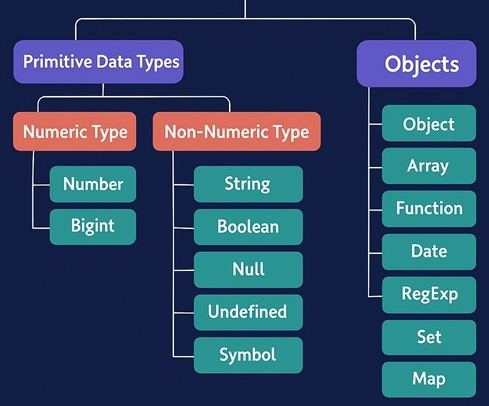
\includegraphics[width=0.5\linewidth]{Images/js_data_types.jpg}
    \caption{JavaScript data types}
    \label{fig:js_data_types}
\end{figure}

To understand the difference between the \texttt{typeof} and \texttt{instanceof} operators, it is important to recall that JavaScript distinguishes between \textbf{primitive values} and \textbf{objects} (see figure \ref{fig:js_data_types}).\\

JavaScript defines the following primitive types:
\begin{itemize}
    \item \texttt{number}
    \item \texttt{bigint}
    \item \texttt{string}
    \item \texttt{boolean}
    \item \texttt{undefined}
    \item \texttt{symbol}
    \item \texttt{null}
\end{itemize}

All other values are objects.

\subsubsection{Understanding the \texttt{typeof} Operator}

The \texttt{typeof} operator returns a string describing the type of a value.

\begin{lstlisting}
// Primitive values
typeof 10.0;            // 'number'
typeof NaN;             // 'number'
typeof 1234n;           // 'bigint'
typeof "Hello";         // 'string'
typeof true;            // 'boolean'
typeof x;               // 'undefined'
typeof Symbol();        // 'symbol'

// Objects
typeof {key:'value'};   // 'object'
typeof [1,2,3];         // 'object'
typeof new Map();       // 'object'
typeof new Set();       // 'object'

// Function
typeof function(){};    // 'function'

// Special case
typeof null;            // 'object'
\end{lstlisting}

\paragraph{Why does \texttt{typeof null} return \texttt{'object'}?}

This is a well-known historical bug in JavaScript. In early implementations, values were represented with type tags, and the tag for objects was \texttt{0}. The value \texttt{null} was represented as a null pointer (\texttt{0x00}), which was mistakenly interpreted as an object.\\

This behavior was never corrected for backward compatibility reasons and remains part of the language.

\subsubsection{Understanding the \texttt{instanceof} Operator}

The \texttt{instanceof} operator checks whether an object is derived from a constructor's prototype.

\begin{lstlisting}
// Objects
let obj = {key:'value'};
obj instanceof Object;      // true

let arr = ['apple', 'orange'];
arr instanceof Object;      // true
arr instanceof Array;       // true

let fun = function(){};
fun instanceof Object;      // true
fun instanceof Function;    // true

let date = new Date();
date instanceof Object;     // true
date instanceof Date;       // true

let regex = /e/;
regex instanceof RegExp;    // true

let set = new Set();
set instanceof Object;      // true
set instanceof Set;         // true

let map = new Map();
map instanceof Object;      // true
map instanceof Map;         // true

// Primitive values
5 instanceof Number;        // false
5 instanceof Object;        // false

// Wrapper objects
let num = new Number(5);
num instanceof Number;      // true
num instanceof Object;      // true
\end{lstlisting}

\subsubsection{Key Differences Between \texttt{typeof} and \texttt{instanceof}}

\begin{itemize}
    \item \texttt{typeof} works on both primitives and objects and returns a string.
    \item \texttt{instanceof} returns a boolean value.
    \item \texttt{instanceof} works only on objects and checks the prototype chain.
    \item \texttt{typeof} is useful for primitive type checking.
    \item \texttt{instanceof} is useful for checking object types and class relationships.
\end{itemize}

\subsubsection{Is \texttt{Object} a superclass in JavaScript?}

JavaScript is not class-based in the same way as Java, but it uses a \textbf{prototype-based inheritance model}.\\

However, in practice:
\begin{itemize}
    \item most objects inherit from \texttt{Object.prototype},
    \item therefore, \texttt{obj instanceof Object} is usually \texttt{true}.
\end{itemize}

This makes \texttt{Object} behave similarly to a superclass, although the underlying mechanism is different.

\subsubsection{Wrapper Objects in JavaScript}

JavaScript provides wrapper objects such as:
\begin{itemize}
    \item \texttt{Number}
    \item \texttt{String}
    \item \texttt{Boolean}
\end{itemize}

These allow primitive values to be temporarily treated as objects. For example:

\begin{lstlisting}
let str = "hello";
str.length; // works due to temporary wrapping
\end{lstlisting}

Using the dot notation to call a method of that primitive data type works because, under the hood, JavaScript creates a temporary and volatile wrapper object containing the same value of the variable. In this example in this specific JavaScript does something like:

\begin{lstlisting}
    new String("hello").length;
\end{lstlisting}

After using the wrapper object, JavaScript destroys it because it is not necessary anymore. This process is called \textbf{autoboxing}.\\

\textbf{Important:}
\begin{itemize}
    \item Primitive values are not objects.
    \item Wrapper objects (e.g., \texttt{new Number(5)}) should generally be avoided.
\end{itemize}

\paragraph{Why should wrapper objects be avoided?}

Although wrapper objects provide a mechanism to treat primitive values as objects, their explicit usage (e.g., \texttt{new Number(5)}, \texttt{new String("hello")}) is generally discouraged for several reasons.

\begin{itemize}
    \item \textbf{Unexpected behavior in comparisons:} Wrapper objects are fundamentally different from primitive values. This can lead to unintuitive results when using comparison operators.

\begin{lstlisting}
let a = 5;
let b = new Number(5);

a == b;   // true
a === b;  // false
\end{lstlisting}

The strict equality operator returns \texttt{false} because \texttt{a} is a primitive value while \texttt{b} is an object.

    \item \textbf{Incorrect boolean evaluation:} All objects in JavaScript are truthy (this topic will be discussed later), regardless of their internal value. This can lead to logical errors.

\begin{lstlisting}
if (new Boolean(false)) {
    console.log("This will be executed");
}
\end{lstlisting}

Even though the wrapped value is \texttt{false}, the condition evaluates to \texttt{true} because the object itself is truthy.

    \item \textbf{Unnecessary overhead:} Wrapper objects introduce additional complexity compared to primitive values. They include internal properties and a prototype chain, which makes them heavier than primitives in terms of memory and execution overhead.

    \item \textbf{Temporary vs explicit wrapping:} JavaScript already performs automatic wrapping (autoboxing) when needed. Explicitly creating wrapper objects is therefore redundant and may introduce confusion.

    \item \textbf{Loss of simplicity and readability:} Using primitives keeps the code simpler and more predictable, while wrapper objects introduce behaviors that are not immediately obvious.
\end{itemize}

In practice, primitive values should always be preferred over their corresponding wrapper objects. Wrapper classes exist mainly for internal use by the language (via autoboxing) and for historical reasons, rather than for direct use in application code.

\section{Control Flow Statements}

Control flow statements allow you to direct the execution path of your code. Their syntax is virtually identical to that of languages like C and Java.

\subsection{Conditional Statements}

\textbf{Conditional Statements (}\texttt{\textbf{if/else}}\textbf{, } \texttt{\textbf{switch}}\textbf{)} execute a block of code only if a specified condition is met.

\paragraph{if / else Statements:} Executes code based on a condition.

\begin{lstlisting}
    if (score >= 90) {
        console.log("Grade: A");
    } else if (score >= 70) {
        console.log("Grade: B");
    } else {
        console.log("Grade: C");
    }
\end{lstlisting}

\paragraph{switch Statement:} Chooses between multiple cases.

\begin{lstlisting}
    switch (day) {
        case 1: console.log("Monday"); break;
        case 2: console.log("Tuesday"); break;
        default: console.log("Other day");
    }
\end{lstlisting}

\subsection{Loop Statements}

\textbf{Loop Statements (}\texttt{\textbf{while}}\textbf{, } \texttt{\textbf{do-while}}\textbf{, } \texttt{\textbf{for}}\textbf{)} execute a block of code repeatedly as long as a condition remains true or for a specified number of iterations.

\paragraph{while Loop:} Repeats code as long as a condition is true.

\begin{lstlisting}
    while (x < 10) {
        x++;
    }
\end{lstlisting}

\paragraph{do-while Loop:} Repeats code as long as a condition is true but the condition is checked at the end of the first iteration.

\begin{lstlisting}
    do {
        x++;
    } while (x < 3);
\end{lstlisting}

\paragraph{for Loop:} Repeats code a set number of times.

\begin{lstlisting}
    for (let i = 0; i < 5; i++) {
        console.log(i);
    }
\end{lstlisting}

\subsection{Truthy and Falsy Values}

In JavaScript, truthy and falsy values are concepts related to implicit boolean evaluation. Every value can be converted to either \texttt{true} or \texttt{false} when used in a boolean context (e.g., conditionals or logical expressions).\\

A \textbf{truthy value} is a value that evaluates to \texttt{true}, while a \textbf{falsy value} evaluates to \texttt{false}. Any value that is not explicitly falsy is considered truthy.

\subsubsection*{Truthy Values}

The following are examples of truthy values:

\begin{itemize}
    \item \texttt{true}
    \item Non-zero numbers: \texttt{1}, \texttt{-1}, \texttt{10.0}
    \item Non-zero BigInt values: \texttt{10n}
    \item Non-empty strings: \texttt{"Hello"}, \texttt{"0"}, \texttt{" "}
    
    Note that:
    \begin{itemize}
        \item \texttt{"0"} is truthy because it is a non-empty string,
        \item \texttt{" "} (a space) is also truthy because it is not empty.
    \end{itemize}

    \item Objects: \texttt{\{key: "value"\}}, \texttt{\{\}}
    \item Arrays: \texttt{[1,2,3]}, \texttt{[]}
    \item Functions: \texttt{function() \{\}}, arrow functions, etc.
    \item Dates: \texttt{new Date()}
    \item Symbols: \texttt{Symbol()}
\end{itemize}

\textbf{Important:} All objects are truthy, even if they are empty.

\subsubsection*{Falsy Values}

JavaScript has a small and well-defined set of falsy values:

\begin{itemize}
    \item \texttt{false}
    \item \texttt{0} and \texttt{-0}
    \item \texttt{0n} (BigInt zero)
    \item \texttt{""} (empty string)
    \item \texttt{null}
    \item \texttt{undefined}
    \item \texttt{NaN}
    \item \texttt{document.all}
\end{itemize}

\paragraph{Why is \texttt{document.all} falsy?}

\texttt{document.all} is a legacy feature introduced for compatibility with very old browsers. It behaves like an object, but it is treated as falsy for historical reasons. Additionally, \texttt{typeof document.all} returns \texttt{"undefined"}, making it a special case in the language.

\subsubsection*{Explicit Boolean Conversion}

When in doubt, a value can be explicitly converted to boolean using:

\begin{lstlisting}
Boolean(value)
\end{lstlisting}

or using double negation:

\begin{lstlisting}
!!value
\end{lstlisting}

For example:

\begin{lstlisting}
console.log(Boolean("")); // false
console.log(Boolean(10)); // true

console.log(!!""); // false
console.log(!!10); // true
\end{lstlisting}

\subsubsection{Default Values Using Logical OR (\texttt{||})}

The \texttt{||} operator is commonly used to assign default values when a variable is falsy:

\begin{lstlisting}
let value = "";
let displayValue = value || "Default value";
console.log(displayValue); // "Default value"
\end{lstlisting}

However, this approach may lead to unintended behavior when valid falsy values (such as \texttt{0} or \texttt{""}) are expected.

\subsubsection{Nullish Coalescing vs Logical OR}

Nullish values (\texttt{null} and \texttt{undefined}) are a subset of falsy values.

\begin{lstlisting}
let value = null;
let displayValue = value || "Default value";
console.log(displayValue); // "Default value"

let value2 = "";
let displayValue2 = value2 ?? "Default value";
console.log(displayValue2); // ""
\end{lstlisting}

The \texttt{??} operator only checks for nullish values, while \texttt{||} checks for all falsy values.

This distinction is important when:
\begin{itemize}
    \item \texttt{0} is a valid value (e.g., counters),
    \item \texttt{""} is meaningful (e.g., string building),
    \item only missing values (\texttt{null}/\texttt{undefined}) should trigger a default.
\end{itemize}

\subsubsection{Safe Property Access}

Truthy/falsy checks can be used to avoid runtime errors:

\begin{lstlisting}
let object = {};

if (object && object.field) {
    console.log("Object and field exist");
} else {
    console.log("At least one of the two does not exist");
}
\end{lstlisting}

In this example:
\begin{itemize}
    \item \texttt{object} is truthy,
    \item \texttt{object.field} is \texttt{undefined} (falsy),
\end{itemize}

so the condition evaluates to \texttt{false}.

\subsubsection{Avoiding Explicit Comparisons}

Truthy and falsy values allow concise conditions:

\begin{lstlisting}
let variable;

if (!variable) {
    console.log("Value is falsy.");
}
\end{lstlisting}

Here, \texttt{variable} is \texttt{undefined}, which is falsy, so the condition evaluates to \texttt{true}.

\chapter{Functions: Reusable Blocks of Code}

A function is a reusable block of code designed to perform a specific task. In JavaScript, functions are "first-class citizens," which means they are treated like any other object. They can be assigned to variables, passed as arguments to other functions, and returned from other functions.

\section{Function Definition and Usage}

There are two primary ways to define a function: as a declaration or as an expression.

\begin{enumerate}
    \item
    \textbf{Function Declaration:} This is the traditional way to define a named function.
    
    \item
    \textbf{Function Expression:} This involves creating a function (often anonymous) and assigning it to a variable.
\end{enumerate}

The key difference between these two forms lies in their \textbf{hoisting} behavior. Function declarations are fully hoisted, meaning they are loaded into memory before any code is executed and can be called before they appear in the code. In contrast, with function expressions, only the variable declaration (\texttt{var greet}) is hoisted (and initialized with \texttt{undefined}), not the function assignment itself. Calling the function before the assignment line will result in an error. \\

Because functions are objects in JavaScript, they can be passed as arguments to other functions. A function that is passed as an argument to another function is known as a \textbf{callback function}. The outer function can then invoke this callback to complete a routine or action at the appropriate time. \\

For example:

\begin{lstlisting}
    // Function expression to be used as a callback
    var printMessage = function(max) {
        var message = "";
        for (var i = 0; i < max; i++) {
            message += "hello ";
        }
        return message;
    }
    
    // Function declaration accepting a callback
    function hello(callbackFunc) {
        return "Welcome " + callbackFunc(3);
    }
    
    // Pass printMessage as a callback to the hello function
    hello(printMessage);
\end{lstlisting}

\begin{lstlisting}
    OUTPUT
    Welcome hello hello hello
\end{lstlisting}

This powerful feature of treating functions as data is central to many advanced patterns in JavaScript, especially when working with complex data structures like arrays and objects.

\chapter{Working with Data Structures: Arrays and Objects}

Arrays and objects are the primary data structures for organizing collections of data in JavaScript. Arrays store ordered lists of values, while objects store collections of key-value pairs. Mastering their properties and methods is essential for any form of data manipulation.

\section{Arrays}

A JavaScript array is a structured, ordered sequence of values.

\begin{lstlisting}
    let names = ["Antonio", "Giuseppe", "Cosimo"];
\end{lstlisting}

The key characteristics of an array make it a flexible and powerful tool:

\begin{itemize}
    \item
        \textbf{Dynamic Sizing:} Arrays can grow or shrink at runtime.
        \begin{lstlisting}
            let names = new Array();
            names[0] = "Antonio";
            names[1] = "Giuseppe";
            names[2] = "Cosimo";
        \end{lstlisting}

    \item
        \textbf{Sparse Nature:} Arrays can contain empty slots. Those elements occupy no memory, making arrays efficient for storing data with gaps.
    
    \item
        \textbf{Heterogeneous Elements:} An array can contain elements of mixed data types (e.g., numbers, strings, and even other arrays).
        \begin{lstlisting}
            let colors = ["Yellow", "Red", , , "Blue"];
        \end{lstlisting}
        In this example, the array has 5 elements but the elements with indices 2 and 3 are \textbf{empty slots} (not explicitly assigned). Accessing them returns \texttt{undefined}.
        
        We can also create sparse arrays manually:
        \begin{lstlisting}
            let array_test = new Array();
            array_test[0] = "var";
            array_test[1] = "bar";
            array_test[3] = "filler";
            array_test[4] = "foo";
            
            console.log(array_test); 
            // ['var', 'bar', , 'filler', 'foo']
        \end{lstlisting}
    
    \item 
        \textbf{Nesting possibility:} JavaScript does not have true multidimensional arrays, but it supports \textbf{arrays of arrays}. For example:
        \begin{lstlisting}
            let matrix = [
                [1, 2, 3],
                [4, 5, 6],
                [7, 8, 9]
            ];
            
            matrix[0][1]; // 2
        \end{lstlisting}

        \textbf{Important clarification:} Using multiple indices does not automatically create nested arrays.

        Consider the following experiment:
        \begin{lstlisting}
            let test = ['Top element 0', 'Top element 1', 'Top element 2'];
            
            test[0][0] = 'Nested element 0-0';
            test[0][1] = "Nested element 0-1";
            test[2][2] = "Nested element 2-2";
        \end{lstlisting}

        At first glance, it may seem that we are working with a two-dimensional array. However, this is not the case.

        \begin{itemize}
            \item Each element of \texttt{test} is a \textbf{string}, not an array.
            \item Expressions like \texttt{test[0][0]} are interpreted as:
            \begin{lstlisting}
                ("Top element 0")[0]
            \end{lstlisting}
            \item This means we are accessing a \textbf{character} of a string, not a second dimension.
        \end{itemize}

        \textbf{Important:} Strings in JavaScript are \textbf{immutable}. Therefore, assignments like:
        \begin{lstlisting}
            test[0][0] = 'Nested element 0-0';
        \end{lstlisting}
        do not actually modify the string. The operation is silently ignored, even though the console may display the assigned value.

    \item 
        \textbf{Easy length access:} The \texttt{.length} property returns the number of elements in the array. Consider the following experiment:
        \begin{lstlisting}
            let test = ['Top element 0', 'Top element 1', 'Top element 2'];
            
            test.length;     // 3
            test[0].length;  // 13
            test[2].length;  // 13
        \end{lstlisting}

        \begin{itemize}
            \item \texttt{test.length = 3} because the array contains 3 elements.
            \item \texttt{test[0].length = 13} because \texttt{test[0]} is a string:
            \begin{lstlisting}
                "Top element 0"
            \end{lstlisting}
            which contains 13 characters.
        \end{itemize}

        \textbf{Key takeaway:}
        \begin{itemize}
            \item The \texttt{length} of an array counts its elements.
            \item The \texttt{length} of a string counts its characters.
            \item Accessing \texttt{array[i][j]} only makes sense if \texttt{array[i]} is itself an array.
        \end{itemize}
\end{itemize}

Arrays come with a rich set of built-in methods for manipulation, including:

\begin{itemize} 
    \item
    \texttt{.sort()}: Sorts the elements of an array in place. By default, it sorts alphabetically.

    \item 
    \texttt{.sort(compare\_function)}: Orders the array according to a comparison function between elements defined by the user. For example:
    \begin{lstlisting}
        myArray.sort(function(a, b) { return a - b; })
    \end{lstlisting}
    
    \item
    \texttt{.reverse()}: Reverses the order of the elements of an array in place.
    
    \item
    \texttt{.push()}: Adds one or more elements to the end of an array and increases its size.
    
    \item
    \texttt{.pop()}: Removes the last element from an array and returns that element. This operation reduces the size of the array.

    \item
    \texttt{.toString()}: Returns a string containing the values of the array separated by commas.
\end{itemize}

For iteration, the \texttt{forEach()} and \texttt{map()} methods are particularly useful:

\begin{itemize}
    \item
    \texttt{\textbf{forEach()}}: Executes a provided callback function once for each array element. It does not create a new array and can modify its elements. This method is used in situations in which we don't have to create another array even if we don't have to modify it. 
    
    \item
    \texttt{\textbf{map()}}: Creates a \textbf{new array} populated with the results of calling a provided callback function on every element in the calling array. This is ideal for transforming data from one form to another.
\end{itemize}

\subsection{Example of \texttt{forEach()} usage}

In this example we show the elements contained in an array one by one.

\begin{lstlisting}
    let months = ["Jan", "Feb", "March", "April"];
    months.forEach(function(element, index, array){
        console.log(element.toUpperCase());
    });
\end{lstlisting}

\begin{lstlisting}
    OUTPUT:
        JAN
        FEB
        MARCH
        APRIL
\end{lstlisting}

\noindent
\texttt{Note:} 
    \begin{itemize}
        \item 
        The internal callback function can have at most 3 parameters:
        \begin{enumerate}
            \item \texttt{element}: The value of the current array element;
            \item \texttt{index}: The index of the current array element;
            \item \texttt{array}: A reference to the whole array. This value is useful if we want to modify the original array elements.
        \end{enumerate}

        \item
        JavaScript has a placeholder character so calling functions ignoring a parameter is possible. It is possible to call the \texttt{forEach()} function as follows:
        \begin{lstlisting}
            let months = ["Jan", "Feb", "March", "April"];
            months.forEach(function(_, index, array){
                console.log(array[index].toUpperCase());
            });
        \end{lstlisting}
    \end{itemize}


\subsection{Example of \texttt{map()} usage}

This example is similar to the previous one: given an array of months we create another array containing the name of the months in upper case.

\begin{lstlisting}
    let months = ["Jan", "Feb", "March", "April"];
    let newMonths = months.map( function(element, index, array){
        return element.toUpperCase();
    });
\end{lstlisting}

\begin{lstlisting}
    OUTPUT:
        newMonths = ["JAN", "FEB", "MARCH", "APRIL"]
\end{lstlisting}

Notice that the internal callback function has the same parameters as the internal callback function of the \texttt{forEach()} method but, unlike the previous method, the \texttt{map()} method returns a new array. In fact, the internal callback function of this method has a return statement and the returned value is store in a variable.\\

To better understand what \texttt{map()} does, consider its conceptual equivalent written as a \texttt{for} loop:

\begin{lstlisting}
    // This for loop demonstrates what the map() method does internally.
    let originalArray = [1, 2, 3];
    let newArray = [];
    
    for (let i = 0; i < originalArray.length; i++) {
        // A function is applied to each element, and the result is pushed to the new array.
        newArray.push(originalArray[i] * 2);
    }
    // newArray is now [2, 4, 6]
\end{lstlisting}

\section{Objects}

A JavaScript object is an unordered collection of key-value pairs, where keys are strings or Symbols, and values can be any data type.\\

Objects are typically created using object literal syntax. Properties can be accessed using either dot notation or bracket notation.

\begin{lstlisting}
    // Creating an object literal
    let person = {
      name: "Alice",
      age: 30,
      isStudent: false,
      greet: function() {
        console.log("Hello, " + this.name);
      }
    };
    
    // Accessing properties
    console.log(person.name);       // Outputs: Alice (dot notation)
    console.log(person["age"]);   // Outputs: 30 (bracket notation)
    
    // Calling an object's method
    person.greet();                 // Outputs: Hello, Alice
    
    // Deleting a property
    delete person.isStudent;
    console.log(person.isStudent);  // Outputs: undefined
\end{lstlisting}

\subsection{Creating an object}

In JavaScript, objects can be created in 3 ways:
\begin{enumerate}
    \item
    \textbf{Using an object constructor:} An object constructor is a special function with the purpose of creating an initializing an object. For example:
    \begin{lstlisting}
        function Person(n, c){
            // The "this" keyword is mandatory
            this.name = n;
            this.surname = c;
        }
        ...
        let bruce = new Person("Bruce", "Springsteen");
    \end{lstlisting}

    \item
    \textbf{Using an object initializer instruction:} In JavaScript, objects are unordered collections of key-value pairs enclosed in curly braces and can be created this way. For example:
    \begin{lstlisting}
        let obj = {property_1: value_1, property_2: value_2,
        ..., property_n, value_n};
        let victor = {name: "Victor", surname: "Hugo"};
    \end{lstlisting}

    \item
    \textbf{Creating an empty object and assigning properties to it:} In JavaScript, objects are dynamic. We can create them as empty associative arrays and add properties later or we could also remove existing properties as in the fist example of this section. Here is an example of empty object initialization and subsequent assignment:
    \begin{lstlisting}
        let p = new Object();
        p.name = "Floriano";
    \end{lstlisting}
\end{enumerate}

\subsection{Methods}

When a function is stored as a property of an an object, it is called a \textbf{method}. To create a method, we can either create a function internal to the collection in the creation phase as we have seen in the first example of this section or we can add a previously created function dynamically after the creation of the object. Here is an example of the second way:
\begin{lstlisting}
    function setYearOfBirthday(a){
        this.year = a;
    }
    function Person(n){
        this.name = n;
        this.setYear = setYearOfBirthday;
    }
    ...
    let boss = new Person("Bruce Springsteen");
    boss.setYear(1949);
    /*
        Now the boss object has the following properties:
            year = 1949
            name = Bruce Springsteen
    */
\end{lstlisting}

It's important to notice that the assignment that turns the previously created function into a method of the object only uses the identifier of the function \textbf{without the parenthesis!}. This is because we want to assign to the property \texttt{setYear} an handler to the function \texttt{setYearOfBirthday} and not a value returned by the latter. If we used the parenthesis we would have called the function to make it return a value and JavaScript would have raised an error when trying to run the command \texttt{boss.setYear(1949);} saying that \texttt{boss.setYear} is not a function. The value returned by the function \texttt{setYearOfBirthday()} without arguments is \texttt{undefined}.

\subsection{Common objects}

JavaScript has a set of commonly used objects which are listed in table \ref{tab:js_commonly_used_objects}.

\begin{table}[h!]
    \centering
    \begin{tabularx}{\linewidth}{|p{0.15\linewidth}|X|p{0.25\linewidth}|} \hline
        \textbf{Object} & \textbf{Description} & \textbf{Examples} \\ \hline

        \textbf{Object} &
        The base object from which all other objects inherit. &
        \texttt{let obj = new Object();} \\ \hline

        \textbf{Array} &
        A collection of ordered elements indexed by numbers. &
        \texttt{let arr = [1, 2, 3];} \\ \hline

        \textbf{Function} &
        A block of code designed to perform a particular task. &
        \texttt{function myFunc() \{ \}} \\ \hline

        \textbf{Date} &
        Used to work with dates and times. &
        \texttt{let now = new Date();} \\ \hline

        \textbf{RegExp} &
        Represents regular expressions for pattern matching in strings. &
        \texttt{let regex = \string/abc\string/;} \\ \hline

        \textbf{Math} &
        Provides mathematical constants and functions. &
        \texttt{let pi = Math.PI;} \\ \hline
        
        \textbf{JSON} &
        Provides methods for parsing and stringifying JSON data. &
        \texttt{let jsonString = JSON.stringify(obj);} \\ \hline  
    \end{tabularx}
    \caption{Commonly used objects in JavaScript}
    \label{tab:js_commonly_used_objects}
\end{table}

JSON stringification is the process of turning a JSON object into a string:
\begin{lstlisting}
    let json_example = {key:'value', var:undefined, var2:null};
    json_string = JSON.stringify(json_example);
    \\ Prints: '{"key":"value","var2":null}'
\end{lstlisting}

Notice that the undefined value is removed during the stringification process.

When working with object methods, you will frequently encounter the \texttt{this} keyword, which refers to the object a method is being called on. Its behavior, however, can be complex and is a common source of confusion.

\chapter{Advanced Concepts: this and Symbol}

As you progress with JavaScript, you will encounter concepts that, while more complex, are critical for writing robust and modern code. The \texttt{this} keyword and the \texttt{Symbol} data type are two such concepts that solve common but nuanced problems in the language.

\section{The \texttt{this} Keyword: Understanding Context}

The \texttt{this} keyword is one of the most important and, at the same time, most confusing concepts in JavaScript.\\

\textbf{Definition:} The value of \texttt{this} depends on \textbf{how a function is called}, not on where it is defined.

\subsection{Strict mode vs. non-strict mode}

JavaScript has two modes of operation: strict mode and non-strict mode. These modes affect how JavaScript code is executed, and understanding the differences between them is crucial for writing secure and reliable code.

\begin{itemize}
    \item
    \textbf{Strict mode} is a subset of JavaScript that provides better error checking and enforces stricter rules for coding. It was introduced in ECMAScript 5 (ES5), which is the fifth edition of the ECMAScript language specification. When strict mode is enabled, the JavaScript engine checks for syntax errors and runtime errors that would otherwise go unnoticed in non-strict mode. This makes it easier for developers to catch errors early in the development process, resulting in fewer bugs and better code quality.

    \item 
    \textbf{Non-strict mode}, on the other hand, is the default mode of operation in JavaScript. In this mode, the JavaScript engine allows for more flexible coding and provides fewer restrictions. This means that some code that would cause errors in strict mode may execute without any issues in non-strict mode. While this may seem advantageous at first, it can lead to unexpected behavior and security vulnerabilities.
\end{itemize}

To enable strict mode in JavaScript, you simply add the string \texttt{"use strict";} at the beginning of a script or function.\\

To the ends of our exposition, we need to consider that in non-strict mode, the \texttt{this} keyword inside a function that is not invoked as a method of an object refers to the global object. In strict mode, however, the \texttt{this} keyword is undefined in such cases. This helps prevent accidental modification of the global object and makes it easier to write secure code.

\subsection{The "left of the dot" rule}

A useful heuristic to understand \texttt{this} is:

\begin{quote}
\textit{Look at what is to the left of the dot when a function is called.}
\end{quote}

\begin{lstlisting}
let obj = {
    name: "Antonio",
    greet: function() {
        console.log(this.name);
    }
};

obj.greet(); // "Antonio"
\end{lstlisting}

Here:
\begin{itemize}
    \item the function is called as \texttt{obj.greet()}
    \item \texttt{this} refers to \texttt{obj}
\end{itemize}

\subsection{Default binding (global context)}

If a function is called without an object, \texttt{this} refers to the global object (or \texttt{undefined} in strict mode):

\begin{lstlisting}
function show() {
    console.log(this);
}

show(); // window (browser) or undefined (strict mode)
\end{lstlisting}

\subsection{The \texttt{this} problem inside callbacks}

Consider the following example (from the lecture slides):

\begin{lstlisting}
var period = {
    message: "Hello",
    months: ["Jan", "Feb", "March", "April"],
    show: function() {
        this.months.forEach(function(month) {
            console.log(this.message + " " + month);
        });
    }
};

period.show();
\end{lstlisting}

Output:
\begin{lstlisting}
undefined Jan
undefined Feb
undefined March
undefined April
\end{lstlisting}

\textbf{Explanation:}
\begin{itemize}
    \item \texttt{this} inside \texttt{show()} refers to \texttt{period}
    \item but \texttt{this} inside the \texttt{forEach} callback refers to the \textbf{global object}
\end{itemize}

This happens because:
\begin{itemize}
    \item the callback function is called \textbf{without an explicit object}
    \item therefore, it loses the original \texttt{this} binding
\end{itemize}

\subsection{Solutions to preserve \texttt{this}}

\subsubsection{Solution 1: Store \texttt{this} in a variable}

\begin{lstlisting}
var period = {
    message: "Hello",
    months: ["Jan", "Feb", "March", "April"],
    show: function() {
        let _this = this;

        this.months.forEach(function(month) {
            console.log(_this.message + " " + month);
        });
    }
};
\end{lstlisting}

\textbf{Explanation:}
\begin{itemize}
    \item \texttt{\_this} stores the correct reference
    \item closures allow access to it inside the callback
\end{itemize}

\subsubsection{Solution 2: Use \texttt{bind()}}

\begin{lstlisting}
var period = {
    message: "Hello",
    months: ["Jan", "Feb", "March", "April"],
    show: function() {
        this.months.forEach(function(month) {
            console.log(this.message + " " + month);
        }.bind(this));
    }
};
\end{lstlisting}

\textbf{Explanation:}
\begin{itemize}
    \item \texttt{bind(this)} creates a new function
    \item the new function has \texttt{this} permanently bound to \texttt{period}
\end{itemize}

\subsubsection{Solution 3: Use arrow functions (recommended)}

\begin{lstlisting}
var period = {
    message: "Hello",
    months: ["Jan", "Feb", "March", "April"],
    show: function() {
        this.months.forEach((month) => {
            console.log(this.message + " " + month);
        });
    }
};
\end{lstlisting}

Output:
\begin{lstlisting}
Hello Jan
Hello Feb
Hello March
Hello April
\end{lstlisting}

\textbf{Explanation:}
\begin{itemize}
    \item arrow functions do \textbf{not} have their own \texttt{this}
    \item they inherit \texttt{this} from the surrounding scope (lexical scoping)
\end{itemize}

\subsection{Key observations}

\begin{itemize}
    \item \texttt{this} is determined at \textbf{call time}, not at definition time
    \item normal functions have their own \texttt{this}
    \item arrow functions inherit \texttt{this} from the outer scope
    \item callbacks (like in \texttt{forEach}) often lose the original \texttt{this}
\end{itemize}

\subsection{Important takeaway}

\begin{quote}
\textit{In JavaScript, understanding \texttt{this} means understanding how a function is invoked.}
\end{quote}

\section{The Symbol Type: Ensuring Uniqueness}

The \texttt{Symbol} primitive type was introduced to solve a specific problem: \textbf{preventing property key collisions in objects}. When multiple libraries or different parts of a large application add properties to a shared object using string keys, there is a risk that they will accidentally use the same key name and overwrite each other's data. \\

Symbols are guaranteed to be unique, which eliminates this risk.

\begin{itemize}
    \item
    A new Symbol is created by calling \texttt{Symbol()}. Each call produces a new, unique value, even if the descriptive string is the same: \texttt{Symbol('id') !== Symbol('id')}.
    
    \item
    Symbol-keyed properties are "quasi-private." They are not enumerated in \texttt{for...in} loops and are ignored by \texttt{JSON.stringify()} and \texttt{Object.keys()}, making them ideal for storing internal metadata that should not interfere with normal object operations.
\end{itemize}

It is important to distinguish between \texttt{Symbol()} and \texttt{Symbol.for()}:

\begin{itemize}
    \item
    \texttt{\textbf{Symbol()}} always creates a new, unique symbol.
    
    \item
    \texttt{\textbf{Symbol.for("key")}} searches a global symbol registry for a symbol with the given key. If one exists, it returns it; otherwise, it creates a new symbol, adds it to the registry, and then returns it. This allows symbols to be shared across different files or realms.
\end{itemize}

Mastering advanced concepts like \texttt{this} and \texttt{Symbol} empowers developers to write more predictable, maintainable, and collision-free code, which is essential for building complex, scalable applications.

\end{document}